\documentclass[12pt,a4paper]{scrartcl}

\usepackage[sc]{mathpazo}
\usepackage[onehalfspacing]{setspace}
\usepackage[T1]{fontenc}
\usepackage[utf8]{inputenc}
\usepackage[ngerman]{babel}
\usepackage{geometry}
\usepackage{amsmath}
\usepackage{amsfonts}
\usepackage{amssymb}
\usepackage{graphicx}
\usepackage{natbib}
\usepackage[hyphens]{url}
\usepackage[printonlyused, withpage]{acronym}
\usepackage{listings}
\usepackage{color}
\usepackage{beramono}
\usepackage{wrapfig}

\geometry{a4paper, portrait, left=2.5cm, right=2.5cm, top=2cm, bottom=2cm}
\parindent0cm

\pagestyle{headings}

\author{Malte Modrow}

\definecolor{lightgray}{rgb}{.9,.9,.9}
\definecolor{darkgray}{rgb}{.4,.4,.4}
\definecolor{purple}{rgb}{0.65, 0.12, 0.82}

\definecolor{gray}{rgb}{0.4,0.4,0.4}
\definecolor{darkblue}{rgb}{0.0,0.0,0.6}
\definecolor{cyan}{rgb}{0.0,0.6,0.6}

\lstdefinelanguage{JavaScript}{
  keywords={typeof, new, true, false, catch, function, return, null, catch, switch, var, if, in, while, do, else, case, break},
  keywordstyle=\color{blue}\bfseries,
  ndkeywords={class, export, boolean, throw, implements, import, this},
  ndkeywordstyle=\color{darkgray}\bfseries,
  identifierstyle=\color{black},
  sensitive=false,
  comment=[l]{//},
  morecomment=[s]{/*}{*/},
  commentstyle=\color{purple}\ttfamily,
  stringstyle=\color{red}\ttfamily,
  morestring=[b]',
  morestring=[b]"
}

\lstdefinelanguage{XML}{
	morestring=[b]",
  	morestring=[s]{>}{<},
  	morecomment=[s]{<?}{?>},
  	stringstyle=\color{black},
  	identifierstyle=\color{darkblue},
  	keywordstyle=\color{cyan},
  	morekeywords={xmlns,version,type}
}

\lstset{
   backgroundcolor=\color{lightgray},
   extendedchars=true,
   basicstyle=\footnotesize\ttfamily,
   columns=flexible,
   frame=single,
   showstringspaces=false,
   showspaces=false,
   numbers=left,
   numberstyle=\footnotesize,
   numbersep=9pt,
   tabsize=4,
   breaklines=true,
   showtabs=false,
   captionpos=b,
   escapechar=',
   inputencoding=utf8,
   literate={Ö}{{\"O}}1{Ä}{{\"A}}1{Ü}{{\"U}}1{ß}{{\ss}}2{ü}{{\"u}}1{ä}{{\"a}}1{ö}{{\"o}}1{©}{{\copyright}}1
}


\begin{document}
\tableofcontents
\thispagestyle{plain}

\newpage
\section{Einleitung}
\label{sec:einleitung}
\newpage
\section{Windows 8}
\label{sec:windows8}
Seit dem 26. Oktober 2012 ist Microsofts aktuellstes Betriebssystem \glqq Windows 8\grqq\ für die breite Öffentlichkeit verfügbar. Dieses unterscheidet sich grundlegend von seinem Vorgänger \glqq Windows 7\grqq. Microsoft verfolgt mit Windows 8 den Ansatz, das gleiche Betriebssystem sowohl für Desktop- als auch für Tablet-Computer\footnote{Tablet-Computer: kleiner, flacher, tragbarer Computer mit einem Touchscreen. Es wird von nun an, der Einfachheit halber die englische Version \glqq Tablet\grqq\ benutzt.} zu verwenden. Es besitzt nach wie vor den bekannten Desktop von Windows 7. Äußerlich sind hier nur kleine Änderungen vorgenommen worden. So besitzt z.B. der Windows Explorer eine neues, kontextsensitives Ribbon-Menü\footnote{Auch bekannt als Menüband oder Multifunktionsleiste.}. Neu ist hingegen das "Modern User Interface" (Modern UI, früher Metro), eine für Touch-Gesten optimierte Oberfläche. Obwohl die neue Oberfläche für Touch-Gesten optimiert ist, kann sie trotzdem auch mit Maus und Tastatur bedient werden. Es können, im Gegensatz zum Desktop, keine herkömmlichen Programme im Modern UI ausgeführt werden. In der Modern UI Oberfläche laufen nur Programme (Apps), die speziell für Windows 8 entwickelt wurden und über den Microsoft Store (siehe Sektion \ref{subsubsec:store} auf Seite \pageref{subsubsec:store}) erhältlich sind. Es soll nun ein etwas detaillierterer Blick auf die neue Oberfläche und dessen Eigenheiten geworfen werden.
\subsection{Neues Bedienkonzept}
\label{subsec:bedienkonzept}
%gesten charms usw

\subsection{Windows 8 als hybrides System}
\label{subsec:hybrides system}
% touch, vorteile, nachteile
Windows 8 kann sowohl auf herkömmlichen Desktop Computern als auch auf Tablet-Computern eingesetzt werden. 
\subsection{Windows RT}
\label{subsec:winRT}
\subsection{Das Ökosystem}
\label{subsec:ökosystem}
\subsubsection{Microsoft Store}
\label{subsubsec:store}
\subsubsection{xBox}
\label{subsubsec:xbox}
\subsubsection{Windows Phone}
\label{subsubsec:windowsphone}

\newpage
\section{Bildsprache}

\newpage
\section{Konzeption der App}
\label{sec:konzeption}
In diesem Kapitel geht es darum, die Konzeption für eine Windows 8 Nachrichten App darzustellen und zu erläutern. Dabei gilt es darzulegen, warum und mit welchem Hintergrund Entscheidungen zu Gunsten der einen oder der anderen Möglichkeit ausfallen. Dazu müssen zunächst die Ziele der App ausgeführt werden. Anschließend muss sich entschieden werden mit welcher Technologie bzw. Programmiersprache gearbeitet werden soll. Zuletzt wird noch ein detaillierterer Blick auf das Herzstück der App geworfen. Das Navigationskonzept. Hierbei ist eine der wichtigsten Fragen: \glqq Wie kann ich auch bei ggf. großen Datenmengen eine übersichtliche, intuitive Struktur schaffen die sich in das Gesamtkonzept von Windows 8 eingliedert?\grqq  

\subsection{Ziel der App}
\label{subsec:zielderapp}
Das Ziel der zu erstellenden App ist, den Inhalt der ZEIT ONLINE Website auf ansprechende Art und Weise in einer Windows 8 Applikation darzustellen. Das Layout und die Darstellung der Inhalte soll sich an das sogenannte \glqq Look and Feel\grqq\ von Windows 8 anpassen und sich daran orientieren. Der Fokus bei den Inhalten liegt auf den Artikeln selbst und den jeweiligen Aufmacher bzw. Teaser Bildern. Das heißt andere Inhalte wie z.B. Bildergalerien, Infografiken, Blogartikel oder Quizze werden von der App nicht erfasst und nicht dargestellt. Hintergrund ist, die App möglichst einfach zu halten da es in der Fragestellung um die Relation zwischen den Aufmacherbildern und dem dahinter liegenden Artikeltext geht. Die App erhebt in dieser Hinsicht keinen Anspruch darauf, die gesamten redaktionellen Inhalte von \mbox{ZEIT ONLINE} darzustellen, sondern versteht sich eher als explorative Applikation im Sinne der Fragestellung.\\
Der User soll die Möglichkeit haben die standardmäßig vorhandenen Artikeltitel auszublenden um so, wenn gewünscht, einen rein visuellen Eindruck der Artikelbilder zu bekommen. Hierzu soll einen Schalter in der Menüleiste am unteren Bildrand geben. Wenn der User sich im Artikel befindet soll er die Möglichkeit haben die Schriftgröße in gewissen Maß selbst zu bestimmen, da die App eventuell auf Monitoren mit verschieden großen Auflösungen ausgeführt werden wird oder die Sehkraft des Users nicht mehr ausreicht um eine normal große Schrift zu erkennen und zu lesen. So wird in den Artikeln ein gewisses Maß an Barrierefreiheit gewährleistet.\\
Das übergeordnete Ziel der App ist es, eine rudimentäre Nachrichten Applikation für Windows 8 zu erstellen. Gleichzeitig soll eine Umgebung geschaffen werden, die es erlaubt Untersuchungen anzustellen, in wie weit es möglich ist allein durch das Betrachten der Aufmacherbilder auf den Inhalt der jeweiligen Artikel zu schließen (siehe Sektion \ref{subsec:rel_bilder_artikel} auf Seite \pageref{subsec:rel_bilder_artikel}). Außerdem soll die App dazu dienen, zu erforschen, wie eine Nachrichten Applikation in der Modern UI Oberfläche von Windows 8 erstellt wird und welche design- als auch funktionstechnischen Vorgaben von Microsofts vorhanden sind. Sprich, wie eine App mit Nachrichteninhalten nach Microsofts Sichtweise auszusehen hat. 

\subsection{Nativ vs. Web}
\label{subsec:nativ_vs_web}
Vor dem Entwickeln einer Windows 8 App muss sich entschieden werden mit welcher Technologie bzw. mit welcher Programmiersprache entwickelt werden soll. Die Rede ist hier von einer App die in der Modern UI Oberfläche von Windows 8 läuft und für diese konzipiert ist. Das heißt es handelt sich nicht um eine klassische .NET oder WIN32 Anwendung für Windows. Um eine Modern UI App zu entwickeln, müssen zwei Dinge zwingend vorhanden sein. Zum einen Windows 8 selbst und zum anderen wird die neueste Version von Visual Studio, Visual Studio 11\footnote{Visual Studio 2011 war die aktuellste Version beim Erstellen dieser Arbeit.}, benötigt. Visual Studio steht in der Express Version für Windows 8 kostenlos zur Verfügung. Des weiteren muss sich zwischen der nativen Umsetzung und der Implementierung mit Webtechnologien entschieden werden. Es soll zunächst erläutert werden was die beiden Begriffe bedeuten und in welcher Weise und welchem Zusammenhang sie bei der Entwicklung einer Windows 8 Modern UI App üblicherweise gebraucht werden.

\subsubsection{Native App}
\label{subsubsec:nativ}
Der heutige Begriff \glqq native App\grqq\ unterscheidet sich in einigen Punkten von der früheren oder ursprünglichen Verwendung des Begriffs. Früher sprach man von einer nativen App wenn direkt auf die Ressourcen der  Maschine zugegriffen wurde, wie z.B. Maschinencode der direkt von der CPU ausgeführt wird. Heute wird eine App oftmals schon als nativ deklariert, wenn es sich nicht um eine Webapp handelt. Eine sinnige Definition liegt irgendwo zwischen diesen beiden Varianten. Eine App ist dann nativ, wenn sie Geräte- , Betriebssystem- oder Laufzeitumgebungsabhängig ist. Das heisst, sie ist für ein spezielles Gerät entwickelt und kann nur auf diesem ausgeführt werden. Sie kann dabei alle Geräte- oder Betriebssystemspezifischen Funktionen nutzen, es ist jedoch egal wie nah an der Hardware tatsächlich programmiert wurde \citep{OBrian2013}.\\
In Visual Studio können native Windows 8  Apps u.a. mit den Programmiersprachen C++, C\# oder Visual Basic erstellt werden. Für das Design bzw. das Aussehen der App wird die Markupsprache - \ac{xaml} - verwendet. Es gibt zwei Möglichkeiten wie das \ac{xaml} erstellt werden kann. Es kann entweder von Hand geschrieben werden oder man lässt es sich automatisch generieren. Zum automatischen Generieren lassen sich per Drag \& Drop Elemente wie z.B. Buttons und andere Schaltflächen aus einer Werkzeugpalette direkt auf die \glqq App-Leinwand\grqq\ ziehen, sowie verschieben oder nach Belieben anordnen.
%Listing XAML oder Screenshot 



\subsubsection{Webapp}
\label{subsubsec:webapp} 
 
\subsubsection{Windows 8 App mit Webtechnologien}
\label{subsubsec:webwin8}

\subsection{Navigationskonzept}
\label{subsec:navikonzept}
Damit der User ein für ihn angenehmes und flüssiges Nutzungserlebnis hat, ist es notwendig sich über das Navigationskonzept Gedanken zu machen, gerade wenn es sich um eine App handelt, in der es viele verschiedene Inhaltsbereiche gibt. Der User soll sich möglichst intuitiv durch die Inhalte bewegen können. Außerdem muss dem User auf der Einstiegsebene der ein guter Überblick über die vorhandenen Inhalte gegeben werden, damit er von dort aus zielgerichtet weiter navigieren kann, ohne lange suchen zu müssen. Microsoft nennt in seinen Richtlinien für Windows Store Apps (Modern UI Apps) grundsätzlich zwei Möglichkeiten wie die Navigation umgesetzt werden kann.

\subsubsection{Flaches System}
\label{subsubsec:flachessystem}
Das flache Navigationssystem wird in vielen Windows Store Apps verwendet, häufig in Spielen, Browsern oder in Apps zum Erstellen von Dokumenten. Es zeichnet sich dadurch aus, dass sich die Inhalte auf der gleichen hierachischen Ebene befinden. Dieses System eignet sich wenn ein schneller Wechsel zwischen wenigen Seiten oder Registerkarten möglich sein soll \citep{MicrosoftNavidesign2013}.

\begin{figure}[h]	
	\centering
	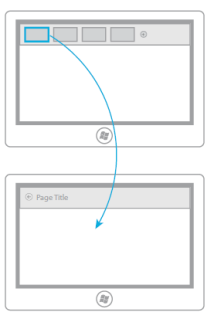
\includegraphics[scale=1]{Bilder/Abbildungen/ms_navigation_flach} 
	\caption{Flaches Navigationssystem \protect\citep{MicrosoftNavidesign2013}.}
	\label{fig:naviflach}
\end{figure}

Abbildung \ref{fig:naviflach} zeigt wie das flache Navigationssystem funktioniert. Am oberen Rand befindet sich eine, nicht immer sichtbare Navigationsleiste mit den verschiedenen Registerkarten oder Seiten. Die Leiste wird angezeigt, wenn der User vom unteren oder oberen Bildrand streift (siehe Sektion \ref{subsec:bedienkonzept}). Wenn der User die Seite wechseln möchte geschieht dies  direkt über die Navigationsleiste, d.h. es gibt meist keinen permananten Zurück-Button. Ein flaches Navigationssystem eignet sich nicht unbedingt für eine Nachrichten App wie die, die in dieser Arbeit konzipiert und umgesetzt ist, weil es zu viele Bereiche (Ressorts) gibt, welche sich zudem sehr ähneln. Hier ist es angebracht ein hierarchisches Navigationssystem zu verwenden.    



\subsubsection{Hierarchisches System}
\label{subsubsec:hierachischessystem}
Die meisten Windows Store-App benutzen ein hierarchisches Navigationssystem. Microsoft nennt es Hubnavigationsmuster. Es eignet sich um große Inhaltssammlungen zu ordnen und sie für User benutzerfreundlich auf zu bereiten. Der Schlüssel dazu ist die Unterteilung des Inhalts in verschiedene Detailebenen \citep{MicrosoftNavidesign2013}.

\begin{figure}[h]	
	\centering
	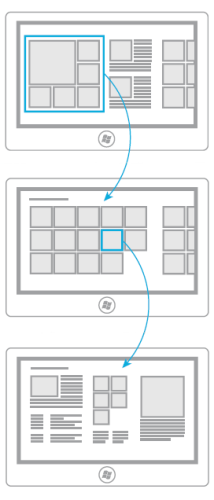
\includegraphics[scale=1]{Bilder/Abbildungen/ms_navigation_hierarchie} 
	\caption{Hierarchisches Navigationssystem \protect\citep{MicrosoftNavidesign2013}.}
	\label{fig:navihierarchisch}
\end{figure}

Das Schema eines hierarchischen Systems ist in Abbildung \ref{fig:navihierarchisch} dargestellt. Der Einstiegspunkt in die App ist die sogenannte \glqq Hubseite\grqq\, hier ganz oben in der Abbildung zu sehen. Auf der Hubebene werden aus den vielen großen Bereichen der App jeweils ein kleiner Teil gesammelt und dargestellt, sodass sich der User vorstellen kann was ihn im jeweiligen Bereich erwartet. Die Anordnung, in welcher der Auszug der Inhalte dargestellt ist muss nicht für jeden Bereich gleich sein. Es kann das Nutzungserlebnis sogar verbessern und vielfältiger machen wenn unterschiedliche Darstellungen (z.B. in Höhe, Breite oder Anzahl der Objekte) für die Bereiche genutzt werden. Die Hubansicht wird horizontal gescrollt, d.h. weiterer Inhalt befindet sich hinter dem rechten Rand und kann entweder durch das Scrollrad der Maus oder auf einem Tablet, durch das swipen nach links in das Sichtfeld des Users gebracht werden.\\
Die mittlere Darstellung in Abbildung \ref{fig:navihierarchisch} zeigt die zweite Detailstufe des hierarchischen Systems. Hier werden alle Elemente eines Bereichs dargestellt. In diesem Fall werden hier alle Artikel aus einem Ressort aufgelistet.\\
Im unteren Bereich der Abbildung ist schließlich die letzte Detailstufe zu sehen. Es handelt sich hierbei um den eigentlichen Inhalt (z.B. einen Artikel). Es ist ebenfalls möglich von der Hubansicht direkt in die Detailansicht eines Elements zu wechseln.  

\begin{figure}[h]	
	\centering
	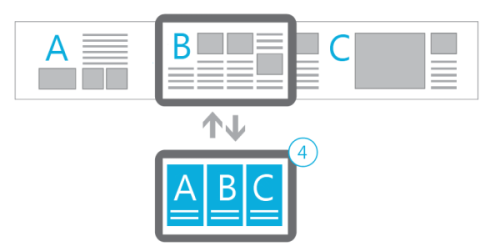
\includegraphics[scale=1]{Bilder/Abbildungen/ms_navigation_hierarchie_semantic_zoom} 
	\caption{Schema des \glqq Semantic Zoom\grqq\ \protect\citep{MicrosoftNavidesign2013}.}
	\label{fig:semanticzoom}
\end{figure}

Befinden sich in der Hubansicht, trotz der Zusammenfassung der Bereiche noch zu viele Bereiche und es dauert zu lange bis zum Ende zu scrollen, kann man noch eine weitere Ebene \glqq davor\grqq\ legen. Das Konzept nennt Microsoft \glqq Semantic Zoom\grqq\ und ist in Abbildung \ref{fig:semanticzoom} schematisch dargestellt. Oben in der Abbildung ist die Hubansicht dargestellt, unten die zusätzliche semantic Zoom Ebene. In der Praxis kann der User auf diese Weise die Inhalte noch weiter vereinfachen und zusammenfassen lassen. Im Fall dieser App soll es einen semantischen Zoom geben, um ein flüssigeres und schnelleres Navigieren z.B. ganz zum Ende der Hubansicht zu ermöglichen, da es über zehn verschiedene Ressorts geben wird. Diese Ansicht soll nur die Namen der verschiedenen Ressorts, sowie ein zufälliges Bild aus dem jeweiligen Ressort zeigen. Um am Desktop-PC (mit Maus) diese Ansicht aufzurufen, muss der User auf ein kleines Minuszeichen am unteren rechten Rand klicken. Am Tablet wird der semantische Zoom mit der \glqq Pinch to Zoom (out)\footnote{Pinch to Zoom erklären}\grqq\  Geste aufgerufen. Klickt der User auf ein Element in dieser zusätzlichen Navigationsebene, wird er direkt zum jeweiligen Ausschnitt in die Hubansicht navigiert. Die semantic Zoom Ansicht kann von überall aus der Hubansicht aufgerufen werden.    


\subsection{Menü und Features}
\label{subsec:menuandproperties}
Da die App einen explorativen Charakter hat wird sich bei den Funktionen und Features auf das nötigste beschränkt. Es soll eine untere App-Leiste geben, in welcher, je nach dem in welcher Ansicht sich der User gerade befindet verschiedene Optionen angezeigt werden. Diese Leiste ist nicht dauerhaft zu sehen und kann, wenn man mit der Maus arbeitet durch einen Rechtsklick aufgerufen werden. Auf einem Tablet geschieht dies durch swipen vom oberen oder unteren Bildschirmrand.\\
In der Startansicht, sowie in der Einzelbereichsübersicht soll es am unteren Bildrand die Möglichkeit geben, die Titel aller Elemente aus- bzw. auch wieder einzublenden um so dem User ein rein visuelles Erleben der Artikelbilder zu ermöglichen. In der Artikelansicht soll der User die Möglichkeit haben, die Schriftgröße des Artikels zu vergrößern, zu verkleinern, sowie die Schriftgröße wieder auf ihren Startwert zu setzen. 

\newpage
\section{Umsetzung der App}
\label{sec:umsetzungderapp}

\subsection{Datenanbindung}
\label{subsec:datenanbindung}
Es soll zunächst geklärt werden wie sich der Inhalt der ZEIT ONLINE Website darstellt und wie er generiert wird. Die redaktionellen Inhalte werden fast ausschließlich über ein hauseigenes \ac{cms} erstellt und gepflegt. Das \ac{cms} generiert aus den Inhalten eine \ac{xml}-Struktur. Aus dem \ac{xml} wiederum wird anschließend mit Hilfe von \ac{xslt} in einer zweistufigen Transformation das fertige \ac{html} erstellt. Dies ist ein grober Überblick wie sich die Webseite von ZEIT ONLINE zusammensetzt.\\
Für die Windows 8 App wird direkt das \ac{xml} verwendet, welches vom \ac{cms} generiert wird. Für die App werden zwei verschiedene Seitentypen der Webseite benötigt um die gewünschten Informationen darzustellen. Zum einen die verschiedenen \glqq Centerpages\grqq\ und zum anderen die Artikelansicht. Centerpages sind die Hauptseiten der jeweiligen Ressorts (z.B. die Hauptseite des Politikressorts), sowie die Startseite mit den wichtigsten und aktuellsten Meldungen. Auf den Centerpages befinden sich die Teaserelemente für die verschiedenen Artikel. Die Teaserelemente bestehen meist aus einem Bild und einem kurzen, prägnanten Text, welcher kurz erläutert worum es in dem dahinter liegenden Artikel geht.\\
%xml des buttons 
\begin{lstlisting}[language= XML,caption=Das XML eines Teaserelements, label={lst:knopfxml}]
<block href="http://xml.zeit.de/digital/internet/2013-08/fablab-open-hardware" year="2013" issue="34" ressort="Digital" author="Tilman Baumgärtel" contenttype="article" publication-date="" expires="" date-last-modified="2013-08-14T12:58:40+00:00" date-first-released="2013-08-14T09:57:43.627551+00:00" date-last-published="2013-08-14T12:59:39.691370+00:00" last-semantic-change="2013-08-14T09:56:40.185797+00:00">
	<supertitle>Open Hardware</supertitle>
	<title>Fab Labs, die Maschinen-Bibliotheken</title>
	<text>
		3-D-Drucker, CNC-Fräsen oder Lasercutter - mit solchen Maschinen sollen Bastler in Fab Labs experimentieren. Immer mehr solcher Werkstätten entstehen nun in aller Welt.
	</text>
	<description>
		3-D-Drucker, CNC-Fräsen oder Lasercutter - mit solchen Maschinen sollen Bastler in Fab Labs experimentieren. Immer mehr solcher Werkstätten entstehen nun in aller Welt.
	</description>
	<byline/>
	<image alt="MakerBot Replicator 2" align="left" title="MakerBot Replicator 2" base-id="http://xml.zeit.de/digital/internet/2013-08/makerbot-cebit-hannover/" type="jpg" publication-date="" expires="">
		<bu>
			Ein MakerBot Replicator 2 auf der diesjährigen Cebit in Hannover
		</bu>
		<copyright>© REUTERS/Fabrizio Bensch</copyright>
	</image>
</block>
\end{lstlisting}


Das \ac{xml} von einem Teaserelement ist in Listing \ref{lst:knopfxml} dargestellt. Es werden jedoch nicht alle Informationen aus dem \ac{xml} verwendet. Die verwendeten Informationen sind das \glqq date-first-released\grqq\ (Zeile 1), der \glqq title\grqq\ (Zeile 3), sowie die \glqq description\grqq\ (Zeile 7) und das \glqq image\grqq\ (Zeile 11). Das \ac{xml} für die Artikelansicht ist ähnlich aufgebaut, nur ist hier zusätzlich noch der Artikeltext (Inhalt) in Form von Paragraphen-Tags (<p>) enthalten. Dies ist ein konkreter Einblick wie die rohen Daten aussehen, welche für die App verwendet werden. Wie die Daten im Detail verarbeitet werden wird in Sektion \ref{subsec:wichtigercode} auf Seite \pageref{subsec:wichtigercode} näher erläutert.

\subsection{Ressort Ansichten}
\label{subsec:ressortansichten}
Wenn die App startet befindet sich der User in der Startansicht. Hier werden ihm für alle Hauptressorts die ersten sechs Artikel angezeigt, in der Reihenfolge wie sie auch auf der Webseite zu finden sind. 

\begin{figure}[h]
	\centering
	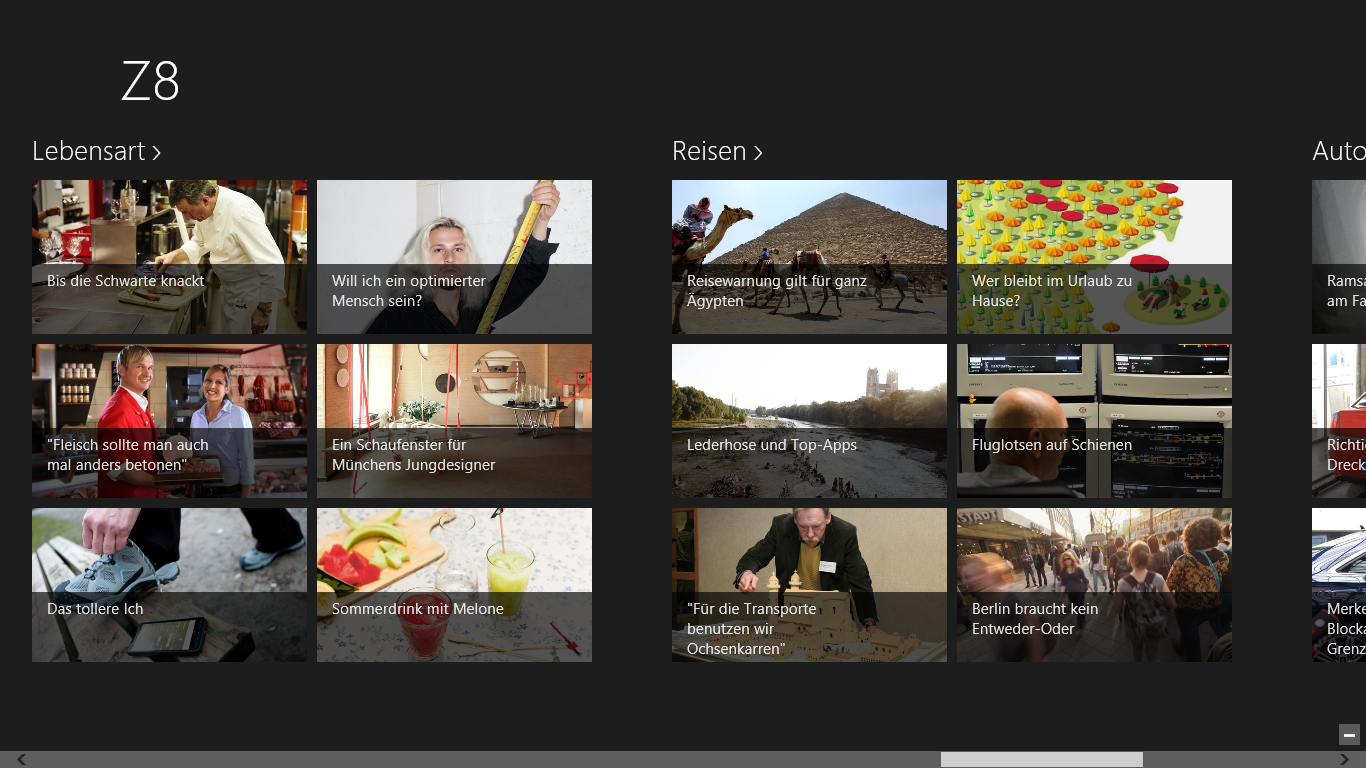
\includegraphics[width=\textwidth]{Bilder/Screenshots/app/reise_aegypten_2gmit.png} 
	\caption{Ressortübersicht in Startansicht.}
\end{figure}


\subsection{Wichtiger Code}
\label{subsec:wichtigercode}



\newpage
\section{Evaluierung} 
\label{sec:evaluierung}
\subsection{Relation Bilder - Artikelinhalt}
\label{subsec:rel_bilder_artikel} 

\newpage
\section{Fazit}
\label{sec:fazit}

\newpage
\section*{Abkürzungsverzeichnis}
\label{sec:abkürzungen}
\begin{acronym}[SEPSEP]
	\acro{xaml}[XAML]{Extensible Application Markup Language}
	\acro{cms} [CMS]{Content Management System}
	\acro{xml} [XML]{Extensible Markup Language}
	\acro{xslt}[XSLT]{Extensible Stylesheet Language Transformations}
	\acro{html}[HTML]{Hypertext Markup Language}
\end{acronym}

\newpage
\begin{singlespace}
	\bibliographystyle{natdin}
	\bibliography{ba_literatur}
\end{singlespace}

\newpage
\listoffigures


\end{document}